%%%%%%%%%%%%%%%%%%%%%%%%%%%%%%%%%%%%%%%%%%%%%%%%%%%%%%%%%%%%%%%%%%%%%%
%%%%%%%%%%  PLANTILLA DE ARTÍCULO DE LA REVISTA TEMAT  %%%%%%%%%%%%%%%
%%%%%%%%%%%%%%%%%%%%%%%%%%%%%%%%%%%%%%%%%%%%%%%%%%%%%%%%%%%%%%%%%%%%%%

% Este archivo puede servir como plantilla a los interesados en presentar artículos a TEMat.
% Hemos intentando dejar claro el uso de los distintos comandos habituales en su uso, así como ejemplos de los más importantes.
% En caso de encontrar errores o tener problemas con las plantillas, por favor, contactad con publicaciones@anemat.com.
\documentclass[bibtex, anon]{TEMat-article}
%% Si estáis enviando el artículo a revisión, cargad la clase de la siguiente manera:
% \documentclass[anon]{TEMat-article}

%% Carga aquí los paquetes extra que quieras, intentando que no se salgan de las recomendaciones...
%% Por ejemplo,
\usepackage{algpseudocode}

\usepackage{standalone}


%Mis paquetes
\usepackage{multirow}
\usepackage{tikz-cd}
\usepackage{braids}

\usetikzlibrary{decorations.shapes}

%%%%%%%%%%%%% PARA USUARIOS DE PSTRICKS Y TIKZ %%%%%%%%%%%%%%%%%
%% Os recomendamos que uséis TikZ, mejor que PSTricks.
%% En cualquier caso, os pedimos que leáis la sección <<Detalles avanzados>> dentro de <<Figuras, dibujos y diagramas>>.
%% de `PlantillaTEMat.tex'.
%%%%%%%%%%%%% Fin para usuarios de PSTricks y TikZ

%Mis comandos
\newcommand{\Z}{\mathbb{Z}}
\newcommand{\R}{\mathbb{R}}
\newcommand{\CC}{\mathbb{C}}


\providecommand{\gene}[1]{\langle{#1}\rangle}


%% Fin del espacio para cargar paquetes.
% Ahora ya empieza el documento en sí.

\title[]{El problema de la palabra en los grupos de trenzas}
% \title[Título corto, opcional]{Título del artículo; escribe el corto si este llega más allá de los 3/4 del ancho de página en las cabeceras}

\author*{Aguilar Martín, Javier}
\email{javiecija96@gmail.com}
\affiliation{Universidad de Sevilla (US)}

%\author*{TEMat, Comité editorial de}
%\email{temat@temat.es}
%\affiliation{Asociación Nacional de Estudiantes de Matemáticas (ANEM)}
%\authornote{Los autores pueden tener notas al pie, por ejemplo, para indicar cambios de afiliación entre la actual y la que se tenía cuando empezó a desarrollarse el trabajo.}
%% Estos nombres son inventados. En nombres de verdad, las partículas del apellido van con el apellido, por supuesto.
%% Se pueden añadir tantos autores como sea necesario.

\msc{20F36}
\keywords{trenzas, grupo, problema de la palabra, algoritmo}
\acknowledgements{Quiero agradecer a mis directores de TFG, Juan González-Menses y Ramón Flores Díaz, por el apoyo y conocimiento aportado que me permitieron desarrollar el trabajo y extraer de él este artículo.}

\addbibresource{plantilla.bib}

\begin{document}
% El resumen debe ser lo último en aparecer antes de empezar con el contenido del artículo.
\begin{abstract}
El problema de la palabra es uno de los problemas más importantes en teoría combinatoria de grupos. En este artículo presentamos una familia de grupos, los grupos de trenzas, donde es posible resolverlo, junto con uno de los algoritmos más eficientes que existen para ello. 
\end{abstract}
\begin{abstract}[english]
The word problem is one of the most important problems in combinatorial group theory. In this paper we present a family of groups, the braid groups, in which it is possible to solve it, together with one of the most efficient algorithms for that purpose.
\end{abstract}
\maketitle

\section{Introducción}
COGER LA BIBLIOGRAFÍA DE MI TFM

El problema de la palabra es uno de los problemas fundamentales de la teoría combinatoria de grupos propuestos por Max Dehn \cite{Dehn11}. Este problema consiste en: dado un grupo $G$ con una presentación finita $\langle S| R\rangle$ y dados dos elementos $a$ y $b$ de $G$ expresados como producto de los elementos de $S$ y sus inversos, decidir si $a=b$ como elementos del grupo o, equivalentemente, si $ab^{-1}=1$.

El nombre de este problema proviene de que podemos considerar el alfabeto $\Sigma=S\cup S^{-1}$, donde $S^{-1}$ representa el conjunto formado por los inversos de los elementos de $S$, y ver $G$ como un lenguaje sobre $\Sigma$, en el que dos palabras $a$ y $b$ representarán el mismo elemento si y solo si se puede transformar $a$ en $b$ mediante un número finito de pasos usando las reglas de reescritura proporcionadas por las relaciones de $R$ junto con la cancelación de inversos.  

El propio Dehn describió algoritmos para resolver el problema de la palabra en grupos fundamentales de 2-variedades orientables cerradas con género mayor o igual que 2 \cite{Dehn12}. Sin embargo, en 1955 Pyotr Novikov encontró ejemplos de grupos finitamente presentados donde el problema de la palabra era indecidible \cite{Novikov}, es decir, que no se puede diseñar un algoritmo que lo resuelva. A pesar de esto, hay gran cantidad de grupos donde el problema de la palabra sí es resoluble. Ejemplos claros de ello son los grupos finitos y los grupos libres. Aquí estudiaremos los grupos de trenzas, que aparecen en numerosas ramas de las matemáticas como el álgebra, la topología y el análisis, y en los cuales el problema de la palabra es resoluble.

PONER ALGO DE LA ESTRUCTURA
%Esta es la plantilla de artículos para la revista TEMat.
%En ella recogemos todas las instrucciones básicas sobre cómo crear artículos en \LaTeX{} de acuerdo a los criterios editoriales de TEMat.
%Hay varios documentos que forman parte de la plantilla.
%Los más importantes son el documento \verb+TEMat-article.cls+, que forma una clase que incluye todo el formato de la revista y \textbf{NO} se debe modificar; el documento \verb+PlantillaTEMat.tex+, que sirve para crear artículos, y el documento \verb+plantilla.bib+, que sirve para crear bibliografías que después se importan al artículo.
%Además, están los archivos \verb+latexmkrc+ (necesario para los que utilicen \verb+latexmk+), y \verb+triangulo.tex+ y \verb+triangulo-ps.tex+ (que proporcionan ejemplos de figuras en \verb+tikz+ y en \verb+pstrics+), así como los diagramas \verb+triangulo-precompilado.pdf+ y \verb+triangulo-ps-precompilado.pdf+ como muestra para la inclusión de figuras.
%Finalmente, el documento \verb+PlantillaTEMat.pdf+ permite ver el resultado después de compilar.
%Si no puedes compilar la plantilla, eso quiere decir que faltan paquetes en tu ordenador, y se deben instalar.
%Si el resultado de la compilación es distinto del ofrecido en el pdf, también hay algún problema.
%Se puede compilar con \verb+pdflatex+, \verb+lualatex+ o \verb+xelatex+ (preferimos uno de los dos primeros, y en principio nosotros compilaremos con el segundo).
%No damos soporte a compilaciones que no sean en modo pdf (\verb|latex+dvips+ps2pdf| u otras).
%
%Esta plantilla (especialmente el documento \verb+TEMat-article.cls+) podría ser revisada y modificada a lo largo del tiempo.
%Recomendamos a los autores que descarguen la versión más reciente de la clase para trabajar.
%En caso de encontrar un error o tener algún problema, contactad con los editores de TEMat a través del correo \email{publicaciones@anemat.com}.

\section{Presentaciones de grupos}

Con la intención de que este texto sea lo más accesible posible, dedicaremos esta sección a explicar qué son las presentaciones de grupos. El lector familiarizado con este concepto puede pasar directamente a la siguiente sección. 

SACARLO DE YAGO

\subsection{Grupos libres}
\begin{definicion}
	Sea $X$ un conjunto, $L$ un grupo e $i:X\to L$ una función. Diremos que $(L,i)$ es \textbf{libre} en $X$ si para todo grupo $H$ y toda función $f:X\to H$ existe un único homomorfismo $\varphi:L\to H$ de modo que el siguiente diagrama conmuta
	\[
	\begin{tikzcd}
	X\arrow[r, "f"]\arrow[d,"i"'] & H\\
	L\arrow[ur, dashed, "\exists!\varphi"']
	\end{tikzcd}
	\]
\end{definicion}

\begin{observacion}\label{4.2}
	Sea $H=\gene{Y}$ un grupo. Sea $X$ un conjunto con $|X|>|Y|$ y $(L,i)$ el grupo libre en $X$. Como $|X|>|Y|$, podemos tomar $f:X\to H$ tal que $Y\subseteq f(X)$. Entonces existe $\varphi:L\to H$ homomorfismo sobreyectivo y tenemos que $H\cong L/\ker\varphi$.
\end{observacion}

\begin{definicion}
	Una \textbf{presentación} de $H$ es un grupo libre $(L,i)$ y un subgrupo $N\trianglelefteq L$ tal que $L/N\cong H$. 
\end{definicion}

\begin{teorema}
	Dado un conjunto $X$, existe $(L,i)$ libre en $X$. SI OCUPA MUCHO DEJARLO SIN PRUEBA Y REFERENCIARLO DEl ENLACE QUE TENGO ABAJO, SI LO DEJO REVISAR LA DEMO
\end{teorema}
\begin{demostracion}
	Sea $X^{-1}$ un conjunto en biyección con $X$ mediante $x\mapsto x^{-1}$. Por abuso de notación a la inversa también la denotamos $x\mapsto x^{-1}$. Sea $(X\cup X^{-1})^*$ el monoide de palabras en $X\cup X^{-1}$ con la yuxtaposición. Decimos que $w=y_1\cdots y_n\in (X\cup X^{-1})^*$ es \textbf{reducida} si $\forall\ 1\leq i\leq n-1$, $y_i\neq y_{i+1}^{-1}$. Si $w$ no es reducida, entonces $w=y_1\cdots y_iy_i^{-1}y_{i+2}\cdots y_n$, se ha obtenido a través de una \textbf{reducción elemental} y ponemos $w\to_r w'$. 
	
	Dos palabras son equivalentes si están en la misma componente conexa del grafo con vértices $V\Gamma=(X\cup X^{-1})^*$ y aristas en las palabras relacionadas por reducciones elementales. 
	
	\[
	\begin{tikzcd}
	zxx^{-}z\arrow[d] & zxx^{-1}y^{-1}y\arrow[l]\arrow[r] &zzy^{-1}y\arrow[lld]\\
	zz 
	\end{tikzcd}
	\]
	
	Entonces se tiene que $F(X)=(X\cup X^{-1})^*/\sim$ es un grupo libre en $X$ y existe una única palabra reducida en cada clase de equivalencia. La segunda afirmación es clara así que vamos a probar la primera. Consideramos $i:X\to F(X)$ la aplicación que envía cada elemento a su clase de equivalencia (de hecho son palabras reducidas). Sea $H$ un grupo y $f:X\to H$ una función. Definimos $\varphi:F(X)\to G$ a partir de las palabras reducidas como $x_{i_1}^{\varepsilon_1}\cdots x_{i_n}^{\varepsilon_n}\mapsto f(x_{i_1})^{\varepsilon_1}\cdots f(x_{i_n})^{\varepsilon_n}$. Cualquier homomorfismo de $F(X)\to G$ que haga que el diagrama conmute debe cumplir esa definición luego es único. Se puede ver con más detalle esta demostración en \url{https://www.math.unl.edu/~mbrittenham2/classwk/990s08/public/myasnikov.1.free.groups.pdf}
	
\end{demostracion}

Volvemos a las presentaciones. Dado $X$, el grupo libre en $X$ existe y es único salvo isomorfismo. Lo denotamos $\gene{X\mid\ }$. 

Dado $R\subseteq G$, $\gene{R^G}$ denota el subgrupo generado por todos los $G$-conjugados de $R$, es decir, $$\bigcap_{N\trianglelefteq G, N\subseteq R} N.$$
Dado un conjunto $X$ y $R\subseteq\gene{X\mid\ }$, denotamos por $\gene{X\mid R}$ al grupo $\gene{X\mid\ }/\gene{R^{\gene{X\mid\ }}}$. Por lo visto anteriormente, para todo grupo $G$ existe un conjunto $X$ y $R\subseteq\gene{X\mid\ }$ tal que $\gene{X\mid R}\cong G$. Veamos algunos ejemplos. 

\begin{ejemplo}\
	\begin{enumerate}[label=\roman*]
		\item Para $n\geq 1$, consideremos la presentación $\gene{x\mid x^n}$. Este es el grupo generado por un elemento de orden $n$, por lo que este grupo es justamente el grupo cíclico $\Z/n\Z$. A menudo, las relaciones se escriben como ecuaciones, de modo que esta presentación podría haberse escrito como $\gene{x\mid x^n=1}$. 
	\item  La presentación del grupo libre abeliano de rango $n$, $\Z^n$, está dada por $\gene{x_1,\dots, x_n\mid [x_i,x_j]=1}$, donde $[x_i,x_j]=x_ix_jx_i^{-1}x_j^{-1}$ es el conmutador de los elementos $x_i$ y $x_j$. Es decir, la presentación expresa que el grupo está generado por $n$ elementos que conmutan entre sí y ninguna relación más, por lo que efectivamente es el grupo libre abeliano de rango $n$. Escribiendo las relaciones como ecuaciones podemos también despejar, y escribir la presentación anterior como $\gene{x_1,\dots, x_n\mid x_ix_j=x_jx_i}$. 
	\end{enumerate}
	\end{ejemplo}

\subsection{Transformaciones de Tietze}

Vamos a concentrarnos a partir de ahora en presentaciones \textbf{finitas}, es decir, tanto $X$ como $R$ serán conjuntos finitos. Se conocen como \textbf{transformaciones de Tietze} los siguientes isomorfismos:
\begin{enumerate}
	\item Si $s\in \gene{R^{\gene{X\mid\ }}}$, entonces $\gene{X\mid R}\cong\gene{X\mid R\cup\{s\}}$.
	\item Si $y\notin X$ y $u\in\gene{X\mid\ }$, entonces $\gene{X\mid R}\cong \gene{X\cup \{y\}\mid R\cup \{yu\}}$.
\end{enumerate}

BUSCARLO PARA REFERENCIARLO
\begin{teorema}
	Si $\gene{X\mid R}\cong\gene{X\mid R'}$ son presentaciones finitas, entonces se puede obtener una presentación de la otra mediante una sucesión finita de transformaciones de Tietze.
\end{teorema}

Por tanto, cualesquiera presentaciones de un grupo son equivalentes, y por tanto tiene sentido hablar de \emph{la} presentación de un grupo. 

Volviendo al problema de la palabra, sea $G=\gene{X\mid R}$ finita y $w\in (X\cup X^{-1})^*$. Entonces $w=_G 1$ si y solo si $w\in \gene{R^{\gene{X\mid\ }}}$ si y solo si $w=\displaystyle\prod_{i=1}^M p_ir_i^{\varepsilon_i}p_i^{-1}$ en $\gene{X\mid\ }$, donde $r_i\in R, p_i\in\gene{X\mid\ }, \varepsilon_i=\pm 1$. EN ALGUNA PARTE TENGO QUE ESCRIBIR LAS NOTACIONES $X^{-1}$ Y LO DEL LENGUAJE COMO ASTERISCO DEL ALFABETO

TENGO QUE HACER ALGUNA INTRODUCIÓN BÁSICA DE HOMOTOPÍA, INCLUYENDO CONCATENACIÓN DE CAMINOS
%Cada artículo tendrá su propia portada (para que se puedan descargar por separado y quede recogida toda la información del artículo en dicha portada), parecida a la de esta plantilla.
%En esta página deberá aparecer toda la información del autor o los autores y del artículo en cuestión.
%Nótese que toda la información se puede introducir antes o después del \verb+\begin{document}+, salvo los resúmenes que deben ir siempre después.
%La portada se genera después de los resúmenes mediante el uso del comando \verb+\maketitle+.
%
%Se debe poner el título del artículo con el comando \verb+\title{}+.
%Si se trata de un título largo (tanto que no cabe en la cabecera de las páginas de la revista), se deberá proporcionar también un título corto.
%Para ello, se deben rellenar los dos campos como sigue: \verb+\title[Título corto, opcional]{Título del artículo}+.
%Se puede ver un ejemplo de esto y de todo lo posterior en el archivo \verb+PlantillaTEMat.tex+ de esta plantilla.
%
%Es necesario incluir el nombre y los apellidos para cada autor, así como su afiliación (en qué universidad (u otro lugar) estudia o trabaja).
%También existe la posibilidad de incluir un correo electrónico, por si alguien quiere contactar al autor para preguntar más sobre el tema, pero poner esto es opcional.
%Para introducir estos datos, se deben utilizar los siguientes comandos:
%\begin{itemize}
%\item \verb+\author{Apellido o Apellidos, Nombre}+ para el nombre (este comando debe ser el primero en aparecer para cada autor);
%\item \verb+\affiliation{Afiliación}+ para indicar la afiliación académica o lugar de trabajo;
%\item \verb+\email{email}+, de forma opcional, para indicar una dirección de correo electrónico de contacto, y
%\item \verb+\authornote{Nota al pie}+, de forma opcional, para añadir una breve nota al pie sobre esa persona.
%\end{itemize}
%En el mundo de las matemáticas, la práctica más habitual es poner a los autores por orden alfabético de apellido, sin darle más énfasis a uno que a los otros, y nosotros aconsejamos esta práctica; sin embargo, mantendremos el orden en que estén en el envío.
%
%Cuando solamente hay un autor, debe usarse el comando \verb+\author*+ (con asterisco) para indicar su nombre. Si hay más de uno, la persona de contacto deberá usar el comando con asterisco y el resto deberán usarlo sin asterisco.
%
%Deberá haber una lista con las palabras clave del artículo, que se debe definir con \verb+\keywords{}+, separándolas por comas (y sin añadir punto final).
%También se debe incluir la clasificación del tema del artículo según la MSC2010 (2010 Mathematics Subject Classification) usando \verb+\msc{}+.
%Para los que no conozcan esto, se debe buscar en la página \url{http://www.ams.org/msc/msc2010.html} el código (o códigos) que mejor se correspondan con la temática del artículo que se presenta.
%De ser posible, se debe poner uno solo; en caso de haber varios temas relacionados, recomendamos que no se pongan más de cinco códigos.
%
%Debajo de esta información aparecen la fecha de recepción y de aceptación del artículo presentado.
%Las que hay en la plantilla están a modo de ejemplo; estos campos los rellenarán los editores de la revista para cada artículo.
%En la versión final de los artículos, aparece también la información bibliográfica del trabajo.
%
%En la misma página aparecerán los agradecimientos (en caso de haberlos), así como las fuentes de financiación (en caso de haberlas).
%Para introducirlas, se utiliza \verb+\acknowledgements{}+.
%
%Finalmente, se debe proporcionar un resumen (o \textit{abstract}) del artículo que se envía. Este resumen debe redactarse tanto en castellano como en inglés.
%Para ello, se define un entorno de resumen delimitado por \verb+\begin{abstract}+ y \verb+\end{abstract}+ para el idioma principal (castellano por defecto) y \verb+\begin{abstract}[english]+ \verb+\end{abstract}+ para inglés.
%El resumen debe aportar información suficiente como para saber de qué trata el artículo y cuáles son las aportaciones principales, pero debe ser lo suficientemente corto como para que no se salga de la portada ninguno de los campos que deben estar en ella.
%
%Una vez se han indicado todos los campos de la portada, debe añadirse el comando \verb+\maketitle+, que aparecerá después de todos ellos y justo antes de empezar con el contenido del artículo.
%
%Para anonimizar el documento para la revisión, basta con cargar la clase \verb+revistaanem+ con la opción \verb+anonimo+ (aunque también \verb+anon+, \verb+anonymous+, \verb+revision+ o \verb+review+).
%Sería así, \verb+\documentclass[anon]{TEMat-article}+
%
%Insistimos: hay ejemplos de todo en \verb+PlantillaTEMat.tex+.
%


\section{Grupos de trenzas}

EN LA BIBLIO TENGO QUE METER MI TFG AUNQUE NO LO CITE, EL COMANDO ANDABA POR LA PLANTILLA

Aunque el término \emph{grupo de trenzas} fue acuñado por Artin en 1925 \cite{ArtinA}, estos grupos ya fueron considerados por Hurwitz en 1891 \cite{Hur} como lo que en terminología moderna se llamaría ``grupo fundamental de espacios de configuración de $n$ puntos en el plano complejo''. Magnus en 1935 \cite{Magnus} consideró el mismo grupo desde el punto de vista de los \emph{mapping class groups}. Markov \cite{Markoff} dio una aproximación totalmente algebraica. 

 Esta variedad de definiciones permite estudiar los grupos de trenzas desde perspectivas muy distintas, lo cual aporta una gran riqueza a la teoría. Aquí veremos la definición más geométrica y mundana, además de su presentación, que también puede tomarse como definición algebraica del grupo.
 
 \subsection{Trenzas como colección de cuerdas}
 Empezamos dando la definición más gráfica e intuitiva, consistente en visualizar las trenzas como cuerdas que se entrelazan. 
 
 \begin{defi}\label{geo}
 	Sea $n\geq 1$ un entero. Denotemos $\Sigma_n$ al grupo simétrico sobre $n$ elementos. Sean $n$ puntos $P_1,\dots, P_n$ en $\CC$ (se puede suponer que $P_k=k$ para todo $1\leq k\leq n$). Se define una \textbf{trenza geométrica de $n$ cuerdas} como una $n$-upla $\beta=(\beta_1,\dots,\beta_n)$ de caminos $\beta_k:[0,1]\to\CC\times[0,1]$ tal que:
 	\begin{itemize}
 		\item $\beta_k(t)=(\alpha_k(t),t)$, donde $\alpha_k(0)=P_k$ para todo $1\leq k\leq n$, 
 		\item existe una permutación $\tau=\tau(\beta)\in\Sigma_n$ tal que $\alpha_k(1)=P_{\tau(k)}$ para todo $1\leq k\leq n$, llamada \textbf{permutación inducida por $\beta$},
 		\item $\alpha_k(t)\neq \alpha_l(t)$ para todo $k\neq l$ y para todo $t\in[0,1]$.
 	\end{itemize}
 	Si la permutación inducida por $\beta$ es el elemento neutro de $\Sigma_n$, es decir, si $\beta_k(1)=(P_k,1)$ para todo $1\leq k\leq n$, entonces decimos que la trenza geométrica es \textbf{pura}.
 	
 	Dos trenzas geométricas $\alpha$ y $\beta$ se dicen \textbf{homotópicas} si existe una familia continua de trenzas $\{\gamma_s\}_{s\in[0,1]}$ de modo que $\gamma_0=\alpha$ y $\gamma_1=\beta$. Es decir, dos trenzas geométricas son homotópicas si son homotópicas como colección de caminos relativamente a los puntos extremos. Consideraremos que dos trenzas geométricas son la misma si son homotópicas, y a la clase de homotopía de una trenza geométrica de $n$ cuerdas la llamaremos \textbf{trenza de $n$ cuerdas}. Nótese que si $\alpha$ y $\beta$ son homotópicas entonces $\tau(\alpha)=\tau(\beta)$, así que diremos que una trenza es \textbf{pura} si los elementos de su clase de homotopía son trenzas geométricas puras.
 \end{defi}

El dibujo tridimensional de una trenza geométrica tiene la siguiente forma:
\begin{figure}[h!]
	\centering
	\includegraphics[scale=0.6]{Imagenes/hilos}
	\caption{Una trenza geométrica pura y una trenza geométrica no pura.}\label{hilos}
\end{figure}

\begin{observacion}
	Para cada $t\in[0,1]$, el plano $\CC\times\{t\}$ es atravesado una sola vez por cada cuerda de la trenza. 
\end{observacion}

Normalmente, se representan las trenzas como su proyección en $\R\times[0,1]$ (posiblemente seguida de una rotación de 90º). Los puntos en los que la proyección de dos cuerdas coincida los representaremos como en la Figura \ref{cruce} para conservar la información de cuál cruzaba originalmente por encima. Salvo homotopía, podemos suponer que la proyección tiene un número finito de puntos de cruce, en los cuales solo intervienen dos cuerdas. Además podemos suponer también que los cruces ocurren a distintas alturas, es decir, para distintos valores de $t\in[0,1]$. En la Figura \ref{plana} se ilustra la proyección de la trenza no pura de la Figura \ref{hilos}. 
\begin{figure}[h!]
	\centering
	
\begin{tikzpicture}
	\braid[ number of strands=3, %lower bound
	border height=2pt,style strands={1}{line width=2pt},style strands={2}{line width=2pt},style strands={3}{draw=none}] (braid) at (1,0)%optional, it's a name
	a_1^{-1};
	\end{tikzpicture}
	
\begin{tikzpicture}
	\braid[ number of strands=3, %lower bound
	border height=2pt,style strands={3}{line width=2pt},style strands={2}{line width=2pt}, style strands={1}{draw=none}] (braid) at (1,0)%optional, it's a name
	a_2;
	\end{tikzpicture}
	
	\caption{Cruce positivo y cruce negativo, respectivamente.}\label{cruce}
	\end{figure}
%Todo artículo debe seguir una estructura que convierta su lectura en algo agradable y permita seguir los argumentos con mayor facilidad.
%Habitualmente, esta estructura se ve reforzada utilizando secciones y subsecciones.
%Para crear una sección basta con usar el comando \verb+\section{nombre}+.
%Para crear subsecciones, se debe usar \verb+\subsection{nombre}+.
%Existe la posibilidad de llegar hasta las subsubsecciones, pero recomendamos encarecidamente que no se haga esto.

REVISAR LA FORMA DE CITAR PARA HACERLO TAL COMO DICE LA PLANTILLA
\begin{defi}\label{estandar}
	Se definen los \textbf{generadores estándar} o \textbf{generadores de Artin} como las trenzas $\sigma_i$ con $1\leq i\leq n-1$ indicadas en la Figura \ref{artingen}.
	\begin{figure}[h!]
		\centering
		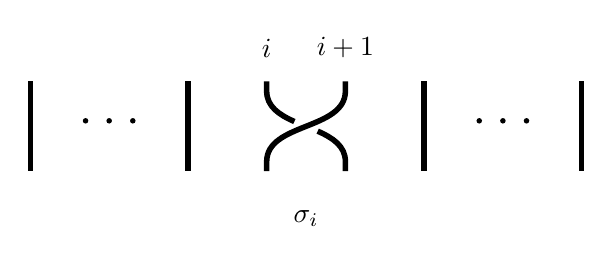
\begin{tikzpicture}
		\fill[black] ( 6.7 , -0.5 ) circle ( 1 pt ) ;
		\fill[black] ( 7 , -0.5 ) circle ( 1 pt ) ;
		\fill[black] ( 7.3 , -0.5 ) circle ( 1 pt ) ;
		
		\fill[black] ( 1.7 , -0.5 ) circle ( 1 pt ) ;
		\fill[black] ( 2 , -0.5 ) circle ( 1 pt ) ;
		\fill[black] ( 2.3 , -0.5 ) circle ( 1 pt ) ;
		\braid[ number of strands=8, %lower bound
		border height=2pt,style strands={8}{line width=2pt}, style strands={7}{draw=none},style strands={6}{line width=2pt},style strands={5}{line width=2pt},style strands={4}{line width=2pt},style strands={3}{line width=2pt}, style strands={2}{draw=none},style strands={1}{line width=2pt}] (braid) at (1,0)%optional, it's a name
		a_4^{-1};
		\node[ at=(braid-4-s),  label=north :  $i$ ] {} ;
		\node[ at=(braid-5-s),  label=north : $i+1$ ] {} ;
		\draw (4.5,-2) node[anchor=south] {$\sigma_i$};
		\end{tikzpicture}
		
		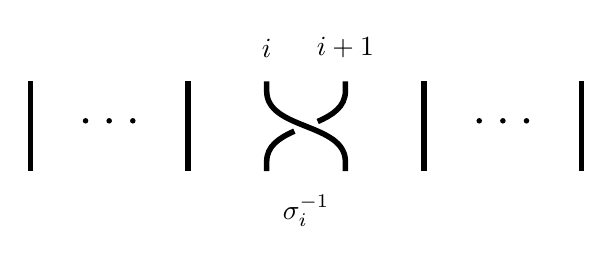
\begin{tikzpicture}
		
		\fill[black] ( 6.7 , -0.5 ) circle ( 1 pt ) ;
		\fill[black] ( 7 , -0.5 ) circle ( 1 pt ) ;
		\fill[black] ( 7.3 , -0.5 ) circle ( 1 pt ) ;
		
		\fill[black] ( 1.7 , -0.5 ) circle ( 1 pt ) ;
		\fill[black] ( 2 , -0.5 ) circle ( 1 pt ) ;
		\fill[black] ( 2.3 , -0.5 ) circle ( 1 pt ) ;
		\braid[ number of strands=8, %lower bound
		border height=2pt,style strands={8}{line width=2pt}, style strands={7}{draw=none},style strands={6}{line width=2pt},style strands={5}{line width=2pt},style strands={4}{line width=2pt},style strands={3}{line width=2pt}, style strands={2}{draw=none},style strands={1}{line width=2pt}] (braid) at (1,0)%optional, it's a name
		a_4;
		\node[ at=(braid-4-s),  label=north :  $i$ ] {} ;
		\node[ at=(braid-5-s),  label=north : $i+1$ ] {} ;
		\draw (4.5,-2) node[anchor=south] {$\sigma_i^{-1}$};
		\end{tikzpicture}
		\caption{Generador de Artin y su inverso.}\label{artingen}
	\end{figure}
\end{defi}\

A partir de las observaciones anteriores, es claro que cualquier trenza se puede construir como concatenación de los generadores de Artin.

\begin{figure}[h!]
	\centering
	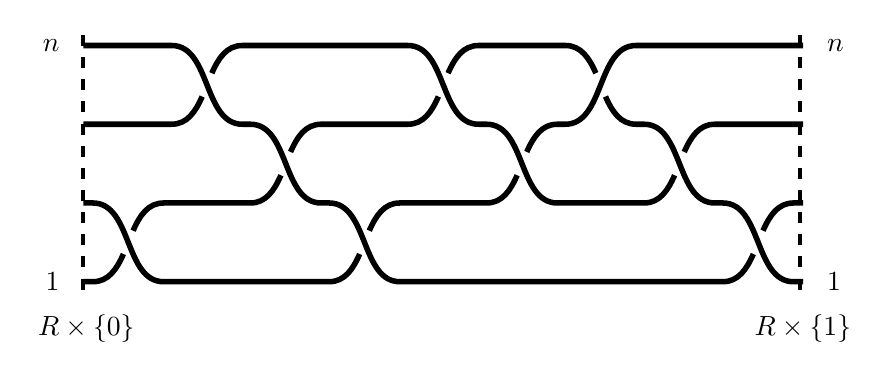
\begin{tikzpicture}
	\draw [line width=1.5pt, dash pattern=on 4pt off 4pt] (0,0.9)-- (0,4.2);
	\draw (-0.7,0.7) node[anchor=north west] {$\mathbb{R}\times\{0\}$};
	\draw [line width=1.5pt, dash pattern=on 4pt off 4pt] (9.1,0.9)-- (9.1,4.2);
	\draw (8.4,0.7) node[anchor=north west] {$\mathbb{R}\times\{1\}$};
	\braid[rotate=90, number of strands=4, %lower bound
	border height=2pt,style strands={1}{line width=2pt},style strands={2}{line width=2pt},style strands={3}{line width=2pt},style strands={4}{line width=2pt}, style floors={1}{dashed}] (braid) at (1,0)%optional, it's a name
	a_1^{-1}a_3^{-1}a_2^{-1}a_1^{-1}a_3^{-1}a_2^{-1}a_3a_2^{-1}a_1^{-1};
	\node[ at=(braid-1-s),  label=west : 1 ] {} ;
	\node[ at=(braid-4-s),  label=west : $n$ ] {} ;
	\node[ at=(braid-1-e),  label=east : 1 ] {} ;
	\node[ at=(braid-2-e),  label=east : $n$ ] {} ;
	\end{tikzpicture}
	\caption{Ejemplo de representación plana.}\label{plana}
\end{figure}
EL DIBUJO DE LA REPRESENTACIÓN PLANA PONERLO MÁS ARRIBA DONDE HABLO DE ELLAS

\subsection{Estructura de grupo}
Una de las características más importantes del conjunto de clases de homotopía de trenzas es que puede dotarse de estructura de grupo para cada $n$. Para ello, definiremos el producto de trenzas. 

\begin{defi}
	El producto de dos trenzas $\alpha=(\alpha_1,\dots, \alpha_n)$ y $\beta=(\beta_1,\dots,\beta_n)$ se define como la trenza
	$$\alpha\cdot\beta = (\alpha_1\beta_{\tau(1)},\dots, \alpha_n\beta_{\tau(n)}),$$
	donde $\tau=\tau(\alpha)$. Es decir, el producto de dos trenzas en el mismo número de cuerdas es su concatenación, en la cual se recorre en primer lugar $\alpha$ y después $\beta$. En la Figura \ref{producto} se ilustra un ejemplo. En ocasiones omitiremos el punto y escribiremos simplemente $\alpha\beta$. Asimismo, denotaremos $\alpha^n=\underbrace{\alpha\cdots\alpha}_{n\text{ veces}}$.
\end{defi}

\begin{figure}[h!]
	\centering
	%\begin{center}
	\resizebox{7cm}{2.cm}{%
		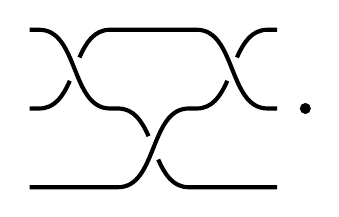
\begin{tikzpicture}
		\braid[ rotate=90, number of strands=3, %lower bound
		border height=2pt,style strands={1}{line width=1.5pt},style strands={2}{line width=1.5pt},style strands={3}{line width=1.5pt}] (braid) at (1,1.5)%optional, it's a name
		a_2^{-1}a_1a_2^{-1};
		\fill[ black ] ( 2 , 2 ) circle (2 pt ) ;
		\end{tikzpicture}
		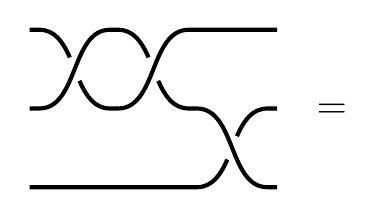
\begin{tikzpicture}
		\braid[ rotate=90, number of strands=3, %lower bound
		border height=2pt,style strands={1}{line width=1.5pt},style strands={2}{line width=1.5pt},style strands={3}{line width=1.5pt}] (braid) at (1,0)%optional, it's a name
		a_2a_2a_1^{-1};
		\draw (3.5,2.2) node[anchor=north west] {\Large=};
		\end{tikzpicture}
	}
	%\end{center}
\end{figure}
\begin{figure}[h!]
	\centering
	\resizebox{10cm}{2.3cm}{%
		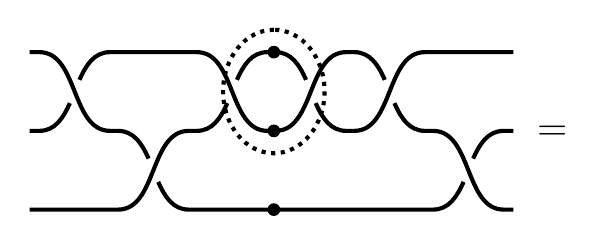
\begin{tikzpicture}
		\braid[ rotate = 90, number of strands=3, %lower bound
		border height=2pt,style strands={1}{line width=1.5pt},style strands={2}{line width=1.5pt},style strands={3}{line width=1.5pt}] (braid) at (1,2)%optional, it's a name
		a_2^{-1}a_1a_2^{-1}a_2a_2a_1^{-1};
		\draw (4.3,2.2) node[anchor=north west] {\Large=};
		\fill[ black ] ( 1.1 , 3 ) circle (2.3 pt ) ;
		\fill[ black ] ( 1.1 , 2 ) circle (2.3 pt ) ;
		\fill[ black ] ( 1.1 , 1 ) circle (2.3 pt ) ;
		\draw [rotate around={90.:(1.1,2.5)},line width=1.5pt,dotted] (1.1,2.5) ellipse (0.7843018170151402cm and 0.6442593318876021cm);
		\end{tikzpicture}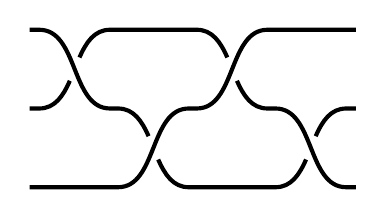
\begin{tikzpicture}
		%\clip (0,-2) rectangle (4, -8);
		\braid[ rotate=90, number of strands=3, %lower bound
		border height=2pt,style strands={1}{line width=1.5pt},style strands={2}{line width=1.5pt},style strands={3}{line width=1.5pt}] (braid) at (1,3)%optional, it's a name
		a_2^{-1}a_1a_2a_1^{-1};
		\end{tikzpicture}
	}
	\caption{Producto de dos trenzas.}\label{producto}
\end{figure}

Denotemos $B_n$ al conjunto de clases de homotopía de trenzas de $n$ cuerdas y $PB_n$ al conjunto de clases de homotopía de trenzas puras de $n$ cuerdas. Es evidente que la multiplicación anterior induce una operación en $B_n$ (y por tanto en $PB_n)$; es más, se tiene el siguiente resultado.

\begin{proposicion}
	El conjunto $B_n$ dotado de esta operación tiene estructura de grupo, y se le llama \textbf{grupo de trenzas de $n$ cuerdas}. El resultado también es cierto para $PB_n$, cuyo nombre es \textbf{grupo de trenzas puras de $n$ cuerdas}. 
\end{proposicion}
REVISAR LA PRUEBA
\begin{demostracion}
	Sean $\alpha$ y $\beta$ dos trenzas con representantes $a=(a_1,\dots, a_n)$ y $b=(b_1,\dots, b_n)$ respectivamente. En primer lugar, veamos que la operación está bien definida, es decir, que $a\cdot b$ es una trenza, y por tanto podemos definir $\alpha\beta=[a\cdot b]$. Sea $\tau=\tau(a)$ la permutación inducida por $a$. Como $a_kb_{\tau(k)}(0)=a_k(0)=(P_k,0)$ para todo $1\leq k\leq n$, se cumple la primera propiedad de la Definición \ref{geo}. Para la segunda, basta observar que la nueva permutación es $\tau(a\cdot b)=\tau(b)\circ \tau(a)$. En particular, si $a$ y $b$ son puras, entonces la permutación inducida por el producto también es la identidad, por lo que el producto es una trenza pura. Por último, si $t\in[0,1/2]$, entonces $a_k\beta_{\tau(k)}=a_k(2t)$ y si $t\in [1/2,1]$, $\alpha_k\beta_{\tau(k)}=\beta_{\tau(k)}(2t-1)$ para todo $1\leq k\leq n$, por lo que se tiene claramente la tercera propiedad. 
	
	Por otra parte, si $a'$ y $b'$ son otros representantes de $\alpha$ y $\beta$ respectivamente, se tiene que $[a'\cdot b']=[a\cdot b]$ por las propiedades de la homotopía de caminos con respecto a la concatenación.
	
	Veamos ahora la estructura de grupo. Tenemos que probar que la operación es asociativa, pero esto se deduce de que la concatenación de caminos es asociativa salvo homotopía.
	Tenemos claramente que la identidad es la trenza constante representada por $Id=(Id_1,\dots, Id_n)$, donde $Id_k$ denota el camino $(P_k, t)$ para $t\in[0,1]$ y para $1\leq k\leq n$.
	Finalmente, dada $\alpha=[(a_1,\dots, a_n)]$ con permutación inducida $\tau$, se tiene que $\alpha^{-1}=[(\overline{a}_{\tau^{-1}(1)},\dots, \overline{a}_{\tau^{-1}(n)})]$, donde $\overline{a}_k$ denota el camino que es opuesto a $a_k$ en la primera coordenada y que es idéntico a $a_k$ en la segunda coordenada. 
	
	En efecto, usando las propiedades de la homotopía de caminos con respecto al camino opuesto:
	\[
	\alpha\alpha^{-1}=[(a_1,\dots, a_n)\cdot (\overline{a}_{\tau^{-1}(1)},\dots, \overline{a}_{\tau^{-1}(n)})]=[(a_1\overline{a}_{\tau(\tau^{-1}(1))},\dots, a_n\overline{a}_{\tau(\tau^{-1}(n))})]=[Id]
	\]
	
	Análogamente se prueba $\alpha^{-1}\alpha=[Id]$. 
	
\end{demostracion}


\begin{figure}[h!]
	\centering
	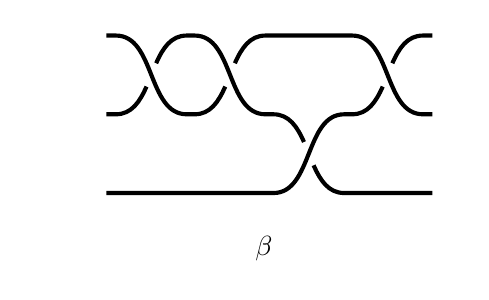
\begin{tikzpicture}
	\clip (0,-1) rectangle (5.5, 2.1);
	\braid[ rotate=90, number of strands=3, %lower bound
	border height=2pt,style strands={1}{line width=1.5pt},style strands={2}{line width=1.5pt},style strands={3}{line width=1.5}, style all floors={}] (braid) at (0,-1)%optional, it's a name
	a_2^{-1}a_2^{-1}a_1a_2^{-1} ;
	\draw (3,-1) node[anchor=south] {$\beta$};
	\end{tikzpicture}
	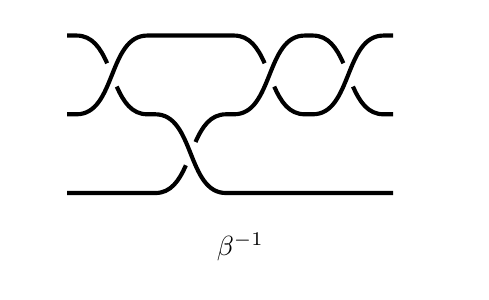
\begin{tikzpicture}
	\clip (0.5,-1) rectangle (6, 2.1);
	\braid[ rotate=90, number of strands=3, %lower bound
	border height=2pt,style strands={3}{line width=1.5pt},style strands={2}{line width=1.5pt}, style strands={1}{line width=1.5pt}] (braid) at (0,-1)%optional, it's a name
	a_2a_1^{-1}a_2a_2;
	\draw (3.2,-1) node[anchor=south] {$\beta^{-1}$};
	\end{tikzpicture}
	\caption{Inversa de una trenza.}\label{especular}
\end{figure}



\subsection{Presentación del grupo}
Una de las características mejor conocidas de los grupos de trenzas es su presentación finita descubierta por Artin en \cite{Artin}. Ya hemos mencionado los generadores $\sigma_1,\dots,\sigma_{n-1}\in B_n$ en la Definición \ref{estandar}. La presentación completa sería la siguiente:
\begin{equation}\label{presentacion}
B_n=\left\langle\begin{array}{c| c c}
\multirow{2}{*}{$\sigma_1,\dots,\sigma_{n-1}$} & \sigma_i\sigma_j=\sigma_j\sigma_i, & |i-j|>1\\
& \sigma_i\sigma_j\sigma_i=\sigma_j\sigma_i\sigma_j, & |i-j|=1
\end{array}\right\rangle.
\end{equation}
La prueba de la completitud de esta presentación puede encontrarse en \cite{Magnus}. 

Vamos a dar también la presentación del grupo de trenzas puras, en concreto la dada por J. S. Birman en \cite{Birman} (ver también \cite{polynomial}), pues nos será más útil para probar ciertos resultados. La presentación original dada por Artin se puede encontrar en \cite{Artin}. Así pues, definimos los \textbf{generadores de Birman}
\begin{equation}\label{birman}
A_{ij}=\sigma_{j-1}\dots\sigma_{i+1}\sigma_i^2\sigma_{i+1}^{-1}\dots\sigma_{j-1}^{-1}\ (1\leq i<j\leq n)
\end{equation}
y las relaciones %n!2(n-1)
\begin{align*}
A_{ij}^{-1}A_{rs}A_{ij}&=A_{rs}\text{ si } (i<j<r<s)\text{ o bien } (r+1<i<j<s),\\
A_{ij}^{-1}A_{js}A_{ij}&=A_{is}A_{js}A_{is}^{-1} \text{ si } (i<j<s),\\
A_{ij}^{-1}A_{is}A_{ij}&=A_{is}A_{js}A_{is}A_{js}^{-1}A_{is}^{-1}\text{ si } (i<j<s),\\
A_{ij}^{-1}A_{rs}A_{ij}&=A_{is}A_{js}A_{is}^{-1}A_{js}^{-1}A_{rs}A_{js}A_{is}A_{js}^{-1}A_{is}^{-1}\text{ si } (i+1<r<j<s).
\end{align*}

En la Figura \ref{generador} se puede observar qué trenza representa geométricamente el generador $A_{ij}$. 

\begin{figure}[h!]
	\centering
	\tikzset{decorate sep/.style 2 args=
		{decorate,decoration={shape backgrounds,shape=circle,shape size=#1,shape sep=#2}}}
	\begin{tikzpicture}
	
	
	
	\node[anchor=south] at (0,2.1) {$j$};
	\foreach \x in {-7,-4,-2,-1,1,4}{
		\draw[white,double=black,very thick,-] (\x,-2) -- (\x,2);
	}
	\draw[white,double=black,very thick,-] (-3,0) -- (-3,2);
	\draw[smooth,white,double=black,line width=2mm,-] plot[variable=\x,domain=-2:2] ({-3.5*exp(-1.4*\x*\x)},{\x});
	\draw[white,double=black,very thick,-] (-3,-2) -- (-3,0);
	\node[anchor=south] at (-3,2.1) {$i$};
	\draw[decorate sep={0.5mm}{9mm},fill] (-6.5,0) -- (-4.5,0);
	\draw[decorate sep={0.5mm}{9mm},fill] (1.5,0) -- (3.5,0);
	\draw[-] (-8,2) -- (5,2);
	\draw[-] (-8,-2) -- (5,-2);
	\end{tikzpicture}
	\caption{Interpretación geométrica de la trenza $A_{ij}$.}\label{generador}
\end{figure}


\begin{nota}
	Cuando $j=i+1$, $A_{ij}=\sigma_i^2$. 
\end{nota}



\section{Algoritmo de Garside}
El objetivo de esta sección será proporcionar una \emph{forma normal} para las trenzas, es decir, una forma ``estándar'' de escribirlas, de modo que para ver si dos palabras representan la misma trenza sea suficiente calcular sus formas normales y comprobar si son iguales. Para llegar hasta esa forma normal estudiaremos la \emph{estructura de Garside} del grupo de trenzas. Los resultados referentes a \emph{Word processing in groups} \cite{Thurston} se pueden encontrar en el capítulo 9 de dicho libro.


\subsection{Formas normales}
Obsérvese que la presentación \ref{presentacion} solo involucra potencias positivas de los generadores. Por tanto, se puede considerar el monoide $B_n^+$ determinado por esa misma presentación. Los elementos de $B_n^+$ son palabras en $\sigma_1,\dots,\sigma_{n-1}$ (pero no sus inversos), y dos palabras son equivalentes si y solo si una puede obtenerse de la otra reemplazando reiteradamente subpalabras de la forma $\sigma_i\sigma_j$ con $|i-j|>1$ (respectivamente, $\sigma_i\sigma_j\sigma_i$ con $|i-j|=1$) por $\sigma_j\sigma_i$ (respectivamente, $\sigma_j\sigma_i\sigma_j$).

\begin{definicion}
	El monoide $B_n^+$ se denomina \textbf{monoide de las trenzas positivas} y sus palabras son llamadas \textbf{trenzas positivas}.
\end{definicion}
En el monoide $B_n^+$ hay un orden parcial natural. 
\begin{definicion}
	Definimos en $B_n^+$ el orden parcial $\preccurlyeq$ tal que dadas $a,b\in B_n^+$, $a\preccurlyeq b$ si $ac=b$ para alguna $c\in B_n^+$. Decimos en ese caso que $a$ es un \emph{prefijo} de $b$. Escribimos $a\prec b$ si $c$ no es trivial. Si además $a\neq 1$, decimos que $a$ es un \textbf{prefijo propio} de $b$. 
\end{definicion}

Antes de continuar debemos probar que la relación que hemos definido es realmente un orden parcial.

\begin{lema}
	La relación $\preccurlyeq$ es una relación de orden.
\end{lema}
\begin{demostracion}
	Dada $x\in B_n^+$ se tiene que $x\preccurlyeq x\cdot 1=x$, por lo que se cumple la propiedad reflexiva. Si $x,y\in B_n^+$ con $x \preccurlyeq y $ e $y \preccurlyeq x$, entonces tenemos que $y=xa$ y $x=yb$ para algunos $a,b\in B_n^+$, así que $y=yba$. Como en el monoide de trenzas positivas las relaciones son homogéneas, tenemos necesariamente que $a=b=1$, por lo que $x=y$, cumpliéndose la propiedad antisimétrica. Por último, supongamos que $x\preccurlyeq y\preccurlyeq z$ para ciertas $x,y,z\in B_n^+$. Entonces $y=xa$ y $z=yb$ para $a,b\in B_n^+$. Sustituyendo, $z=xab$, por lo que $x\preccurlyeq z$, lo que prueba la propiedad transitiva. 
\end{demostracion}
Nótese que $\preccurlyeq$ es invariante por multiplicación a izquierda, esto es, $a\preccurlyeq b$ implica $xa\preccurlyeq xb$ para todo $a,b,x\in B_n^+$. %vale el mismo c

Dado tal orden parcial, uno podría preguntarse si existe un único máximo común divisor o mínimo común múltiplo con respecto a $\preccurlyeq$. Esto es, dadas $a,b\in B_n^+$, ¿existe un único $d\in B_n^+$ tal que $d\preccurlyeq a$, $d\preccurlyeq b$ y $d'\preccurlyeq d$ para todo $d'$ prefijo común de $a$ y $b$? ¿Y existe un único $m\in B_n^+$ tal que $a\preccurlyeq m$, $b\preccurlyeq m$ y $m\preccurlyeq m'$ para todo $m'$ que tenga a $a$ y a $b$ como prefijos? En tales casos, escribimos $d=a\land b$ y $m=a\lor b$. Nótese que también tendríamos $xd=xa\land xb$ y $xm=xa\lor xb$ para todo $x\in B_n^+$.

\begin{nota}
	Análogamente podríamos definir el orden parcial de \emph{sufijos}, $\succcurlyeq$, invariante por multiplicación a derecha. Nótese que este orden no es equivalente al de prefijos, puesto que $b\succcurlyeq a$ no implica en general $a\preccurlyeq b$ ni recíprocamente. Por ejemplo, $\sigma_1\preccurlyeq \sigma_1\sigma_2$, pero claramente $\sigma_1\sigma_2\not\succcurlyeq \sigma_1$.
\end{nota}

El punto clave en el trabajo de Garside fue demostrar mediante métodos elementales que $\sigma_i$ y $\sigma_j$ tienen mínimo común múltiplo en $B_n^+$. En concreto:
\begin{proposicion}(\cite[Teorema 1.2]{Garside})
	El mínimo común múltiplo de los generadores $\sigma_i$ y $\sigma_j$ viene dado por
	$$\sigma_i\lor\sigma_j=\begin{cases}
	\sigma_i\sigma_j & |i-j|>1,\\
	\sigma_i\sigma_j\sigma_i & |i-j|=1.
	\end{cases}$$
\end{proposicion}
%1.2 GARSIDE, la unicidad se ve fácil por la longitud

Garside prueba al mismo tiempo que $B_n^+$ es cancelativo, es decir, $xay=xby$ implica $a=b$ para todo $a,b,x,y\in B_n^+$.

Como las relaciones de \ref{presentacion} son homogéneas, palabras equivalentes en $B_n^+$ tienen la misma longitud, por lo que la longitud de una trenza positiva se define como la longitud de cualquier palabra que la represente. Aunque Garside no lo menciona explícitamente, un argumento inductivo en esta longitud utilizando la cancelatividad permite probar a partir del resultado anterior que todo par de elementos tiene de $B_n^+$ tiene un único mínimo común múltiplo y un único máximo común divisor, tal como se prueba en \cite{Dehornoy}. 
%relaciones homogéneas= LA SUMA DE LOS EXPONENTES A UN LADO Y A OTRO DE LA ECUACIÓN ES LA MISMA
%lo de dehornoy lo tengo en el mismo papel donde me explica el 1.2 de Garside y lo de que los sigma_i son sufijos de Delta. Lo del mcm es lo de las flechitas y el mcd es los bloques

Garside después estudia el siguiente elemento especial.
\begin{definicion}
	La \textbf{trenza fundamental} de $n$ cuerdas es la trenza
	$$\Delta_n=\sigma_1(\sigma_2\sigma_1)\cdots(\sigma_{n-1}\cdots\sigma_1).$$
	Cuando $n$ se sobreentiende, escribimos simplemente $\Delta$. 
\end{definicion} 


\begin{proposicion}\label{conjuga}
	Se verifican: 
	\begin{enumerate}
		\item $\Delta=\sigma_1\lor\dots\lor\sigma_{n-1}$ \cite[Lema 1]{Garside}.
		\item $\sigma_i\Delta=\Delta\sigma_{n-i}$ para todo $i=1,\dots, n-1$ \cite[Lema 4]{Garside}.
	\end{enumerate}
\end{proposicion} 


\begin{figure}[h!]
	\centering
	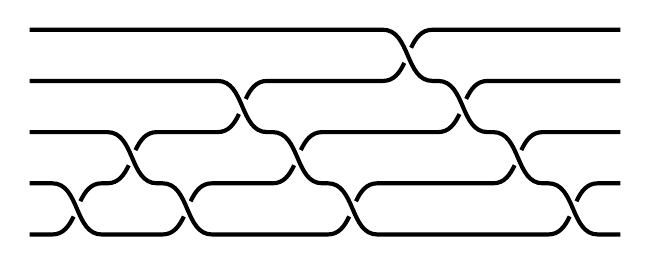
\begin{tikzpicture}
	\braid[rotate=90,width=.65cm,height=0.7cm,line width=1.5pt] s_1^{-1} s_2^{-1} s_1^{-1} s_3^{-1} s_2^{-1} s_1^{-1} s_4^{-1} s_3^{-1} s_2^{-1} s_1^{-1};
	\end{tikzpicture}
	\caption{La trenza fundamental $\Delta_5$.}
\end{figure}


A partir de este resultado podemos deducir las siguientes propiedades sobre $\Delta$.

\begin{proposicion}\label{sufijos} Se cumplen:
	\begin{enumerate}
		\item $\sigma_1,\dots,\sigma_{n-1}$ son también sufijos de $\Delta$.
		\item $\Delta^2$ conmuta con todo elemento de $B_n^+$.
		\item Para todo $a\in B_n^+$ se tiene $a\preccurlyeq\Delta^m$ y $\Delta^m\succcurlyeq a$, donde  $m\geq 0$ es la longitud de $a$.
	\end{enumerate}
	
\end{proposicion}
REVISAR LA DEMO
\begin{demostracion}\
	\begin{enumerate}
		\item En primer lugar, se tiene para $k>i\geq 1$ que $\sigma_i(\sigma_k\cdots\sigma_1)=(\sigma_k\cdots\sigma_1)\sigma_{i+1}$. En efecto, usando las relaciones del monoide de trenzas positivas
		\begin{align*}
		\sigma_i(\sigma_k\cdots\sigma_1)&=\sigma_i(\sigma_k\cdots\sigma_{i+2})(\sigma_{i+1}\sigma_i)(\sigma_{i-1}\cdots\sigma_1)\\
		&=(\sigma_k\cdots\sigma_{i+2})(\sigma_i\sigma_{i+1}\sigma_i)(\sigma_{i-1}\cdots\sigma_1)\\
		&=(\sigma_k\cdots\sigma_{i+2})(\sigma_{i+1}\sigma_i\sigma_{i+1})(\sigma_{i-1}\cdots\sigma_1)\\
		&=(\sigma_k\cdots\sigma_{i+2})(\sigma_{i+1}\sigma_i)(\sigma_{i-1}\cdots\sigma_1)\sigma_{i+i}\\
		&=(\sigma_k\cdots\sigma_1)\sigma_{i+1}.
		\end{align*}
		Así pues, para expresar $\sigma_i$ como sufijo de $\Delta$ hacemos los siguiente. Si $i=1$, entonces por la definición de $\Delta$ ya tenemos que es un sufijo. Si $1<i\leq n-1$, partimos de
		\[
		\Delta=\sigma_1(\sigma_2\sigma_1)\cdots(\sigma_{n-i}\dots\underline{\sigma_1})\cdots(\sigma_{n-1}\dots\sigma_1).
		\]
		Procedemos a desplazar a la derecha el $\sigma_1$ subrayado tal como hemos hecho anteriormente. En cada paso irá aumentando el índice en una unidad. Por tanto, como hay $n-(n-i-1)=i-1$ bloques que se dejan atrás, obtenemos $\sigma_{1+i-1}=\sigma_i$, es decir,
		\[
		\Delta=\sigma_1(\sigma_2\sigma_1)\cdots(\sigma_{n-i}\dots\underline{\sigma_1})(\sigma_{n-i+1}\cdots\sigma_1)\cdots(\sigma_{n-1}\dots\sigma_1)=
		\]
		\[
		\sigma_1(\sigma_2\sigma_1)\cdots(\sigma_{n-i}\cdots\sigma_2)(\sigma_{n-i+1}\cdots\sigma_1\underline{\sigma}_2)\cdots(\sigma_{n-1}\dots\sigma_1)=
		\]
		\[
		\sigma_1(\sigma_2\sigma_1)\cdots(\sigma_{n-i}\cdots\sigma_2)(\sigma_{n-i+1}\cdots\sigma_1)\cdots(\sigma_{n-1}\dots\sigma_1)\underline{\sigma}_i
		\]
		
		
		\item Basta probar que $\Delta^2$ conmuta con $\sigma_i$ para todo $1\leq i\leq n-1$. Como $\sigma_i\Delta=\Delta\sigma_{n-i}$ y $\sigma_{n-i}\Delta=\Delta\sigma_i$ se tiene
		\[
		\sigma_i\Delta^2=\Delta\sigma_{n-i}\Delta=\Delta^2\sigma_i.
		\]
		
		
		\item Probamos $a\preccurlyeq\Delta^m$ donde $m$ es la longitud de $a$ por inducción en $m$. Evidentemente, $1\preccurlyeq\Delta^0=1$. Para una palabra de longitud 1 también es claro porque $\sigma_i\preccurlyeq\Delta$ para todo $1\leq i\leq n-1$ por definición de mínimo común múltiplo. Supongamos ahora, que para una palabra $a\in B_n^+$ de longitud $m-1$ se tiene el resultado. Entonces, cualquier palabra de longitud $m$ será de la forma $\sigma_j a$ para algún $1\leq j\leq n-1$. Así que, usando la invarianza por multiplicación a izquierda y el caso $m=1$,
		\[
		a\preccurlyeq\Delta^{m-1}\Rightarrow \sigma_j a\preccurlyeq \sigma_j\Delta^{m-1} =\Delta^{m-1}\sigma_t\preccurlyeq \Delta^{m-1}\Delta=\Delta^{m}
		\]
		donde $t=j$ o bien $t=n-j$ dependiendo de la paridad de $m$. De forma análoga usando la invarianza por multiplicación a derecha se prueba que $\Delta^m\succcurlyeq a$.
	\end{enumerate}
	
\end{demostracion}


% el a<\Delta^m es cuestión de que como \sigma_i<\Delta, luego ya solo hay que ir multiplicando a izquierda por el sigma_j correspondiente -> \sigma_j\sigma_i<\sigma_j\Delta<\Delta^2, etc El otro igual usando la multiplicación a la derecha

Esto tiene importantes implicaciones. Como todo par de elementos de $B_n^+$ tiene un múltiplo común y $B_n^+$ es cancelativo, las condiciones de Ore (\ref{condiciones}) implican que $B_n^+$ se inyecta en su grupo de fracciones, que es precisamente $B_n$. Por lo tanto, $B_n^+$ no es solamente un monoide definido algebraicamente, sino que puede ser considerado como un submonoide de $B_n$ formado por las trenzas que pueden ser escritas solo con potencias positivas de los generadores. TENGO QUE ESCRIBIR LAS CONDICIONES DE ORE EN ALGÚN LADO

Las propiedades anteriores implican que el orden parcial $\preccurlyeq$ (respectivamente, $\succcurlyeq$) puede ser extendido a $B_n$ de la siguiente manera: dadas $a,b\in B_n$, $a\preccurlyeq b$ (resp. $a\succcurlyeq b$) si $ac=b$ (resp. $b=ca$) para algún $c\in B_n^+$. Esto da un orden parcial que es invariante por multiplicación a izquierda (resp. a derecha), y el cual admite un único mínimo común múltiplo y un único máximo común divisor. Este hecho podrá ser probado una vez definida la \emph{forma normal de Garside} en la sección a continuación.
% a,b\in B_n, a<b sii a^{-1}b\in B_n^+




\subsection{Solución al problema de la palabra}
QUIZÁ ESCRIBIR EL ALGORITMO CON EL ENTORNO DE ALGORITMO DE LA PLANTILLA 

Garside dio una nueva solución al problema de la palabra en los grupos de trenzas de la siguiente manera. Recordemos que para todo $i=1,\dots, n-1$ se tiene que $\Delta\succcurlyeq\sigma_i$ por la Proposición \ref{sufijos} apartado 1, esto es, $\Delta=X_i\sigma_i$ para algún $X_i\in B_n^+$. Dada una trenza escrita como una palabra en $\sigma_1,\dots,\sigma_{n-1}$ y sus inversos, se puede reemplazar cada aparición de $\sigma_i^{-1}$ por $\Delta^{-1}X_i$. Conjugar una trenza positiva por $\Delta$ sigue dando una trenza positiva por la Proposición \ref{conjuga} apartado 2, así que podemos mover todas las apariciones de $\Delta^{-1}$ a la izquierda, de la siguiente forma: si encontramos $\sigma_j\Delta^{-1}$ ($1\leq j\leq n-1)$, entonces por \ref{conjuga} sabemos que $\Delta\sigma_{j}=\sigma_{n-j}\Delta$, si y solo si  $\sigma_j\Delta^{-1}=\Delta^{-1}\sigma_{n-j}$, por lo que podemos sustituir $\sigma_j\Delta^{-1}$ por $\Delta^{-1}\sigma_{n-j}$. Esto muestra que toda trenza puede ser escrita como $\Delta^p A$ para algún $p\in\Z$ y algún $A\in B_n^+$. Además, si $\Delta\preccurlyeq A$, podemos reemplazar $\Delta^p$ por $\Delta^{p+1}$ y $A$ por $\Delta^{-1}A$. Esto reduce la longitud de $A$, así que solo puede hacerse una cantidad finita de veces. Por tanto, toda trenza puede descomponerse \emph{de manera única}, como $\Delta^pA$, donde $p\in\Z$, $A\in B_n^+$ y $\Delta\not\preccurlyeq A$. Efectivamente, si tuviéramos dos expresiones $\Delta^pA=\Delta^q B$ con $p<q$ en las condiciones anteriores, dividiendo por $\Delta^p$ tendríamos que $A=\Delta^{q-p}B$, lo cual contradice el hecho de que $A$ no tenga a $\Delta$ como prefijo. Análogamente para $p>q$, luego $p=q$ y $A=B$.

%\Delta c=A, \Delta^p A = \Delta^{p+1} \Delta^{-1}A=\Delta^{p+1}c
\begin{definicion}
	En base a lo comentado en el párrafo anterior, definimos la \emph{forma normal de Garside} de una palabra $w\in B_n$ como $w=\Delta^pA$, donde $p\in\Z$, $A\in B_n^+$ y $\Delta\not\preccurlyeq A$. 
\end{definicion}

Esta forma normal permite resolver el problema de la palabra, ya que se pueden enumerar todas las palabras positivas que representan la trenza positiva $A$ reiterando las relaciones del monoide de trenzas positivas de todas las formas posibles. Esta fue la solución dada por Garside en \cite{Garside}. Sin embargo, no es muy satisfactoria, ya que da lugar a un algoritmo altamente ineficiente.

El-rifai y Morton \cite{EM} lo mejoraron definiendo la \emph{forma normal a la izquierda} de una trenza. Basta tomar la descomposición $\Delta^pA$ y después definir %izquierda porque se van pasando elementos a la izquierda
\begin{align*}
&a_1=A\land\Delta\\
&a_i=(a_{i-1}^{-1}\cdots a_1^{-1}A)\land\Delta,\ \forall\ i>1.
\end{align*}
Nótese que existe un $r\geq 0$ tal que $a_i=1$ para todo $i>r$, ya que la longitud de $a_{i-1}^{-1}\cdots a_1^{-1}A$ es estrictamente decreciente. De esta forma, toda trenza puede ser escrita de manera única como:
%la longitud decrece porque estás cancelando prefijos de A, luego cada vez lo haces más corto
$$\Delta^p a_1\cdots a_r,$$
donde los $a_i$ son los definidos anteriormente, los cuales por definición son un prefijos propios de $\Delta$, es decir, $1\prec a_i\prec\Delta$, y además se puede demostrar que $(a_ia_{i+1})\land\Delta=a_i$ \cite{Thurston} para todo $i=1,\dots, r-1$. Esta es la anteriormente mencionada forma normal a la izquierda de la trenza. Los prefijos positivos de $\Delta$ son llamados \emph{elementos simples} o \emph{trenzas de permutación}. El nombre no es casual, ya que como prueba Thurston \cite{Thurston}, estas trenzas son justamente las mismas trenzas de permutación definidas en \ref{simples}. Por tanto, la forma normal a la izquierda de una trenza es una descomposición única como producto de una potencia de $\Delta$ y una sucesión de elementos simples propios. Thurston \cite{Thurston} mostró que esta forma normal puede ser calculada en tiempo $O(l^2n\log(n))$ para una palabra de $l$ letras en $B_n$. 

%prefijo propio de Delta porque Delta no era prefijo de A y se está haciendo el meet

En \cite{Thurston} se puede encontrar además una forma más práctica de llevar a cabo el algoritmo de encontrar la forma normal a la izquierda, la cual será la que utilicemos en el ejemplo \ref{ejnormal}. Antes de explicarla vamos a introducir algo de nomenclatura. Dadas dos trenzas simples positivas $A$ y $B$, decimos que un prefijo no trivial $b\preccurlyeq B$ \emph{se puede pasar} de $B$ a $A$ si $Ab$ es simple, y en tal caso \emph{pasar} $b$ de $B$ a $A$ consiste en las transformaciones $A\to Ab$ y $B\to b^{-1}B$. Con esto presente, el algoritmo consiste en lo siguiente:
\begin{enumerate}
	\item Una vez tenemos una palabra $w\in B_n$ en forma normal de Garside $w=\Delta^p A$, si $A=1$, entonces no hay nada que hacer. En caso contrario, dividimos $A$ en bloques formados por elementos simples, digamos, $$A=a_{1,0}a_{2,0}\dots a_{m,0}.$$
	\item En el paso $t\geq 0$ tenemos $A$ expresada en bloques de elementos simples como
	$$A=a_{1,t}a_{2,t}\dots a_{m,t}.$$
	En este paso buscamos el primer par $a_{i,t}a_{i+1,t}$ de modo que se pueda pasar algún prefijo de $a_{i+1,t}$ a $a_{i,t}$ y lo pasamos. Esto nos dará la descomposición 
	$$A=a_{1,t+1}a_{2,t+1}\dots a_{m,t+1}.$$
	\item Volvemos paso 2 y reiteramos hasta que no quede ningún par que verifique la condición. 
\end{enumerate} 

Este proceso naturalmente termina porque el vector formado por las longitudes de los bloques aumenta en cada paso su orden lexicográfico, el cual está acotado por $(m,0,\dots, 0)$ donde $m$ es la longitud de $A$. La forma normal a la izquierda se obtendrá eliminando los bloques triviales (que necesariamente estarán al final). %porque siempre se puede pasar una palabra no vacía a un bloque vacío

Alternativamente, podríamos empezar con una descomposición $w=\Delta^qA$ con $A\in B_n^+$, pero sin asegurarnos de que $\Delta \not\preccurlyeq A$, pues $\Delta$ aparecería al acumular elementos simples en caso de ser prefijo de $A$, y podríamos enviarlo al bloque de $\Delta^q$. En cualquier caso, este proceso acabará con la forma normal a la izquierda, pues no poder pasar ninguna letra del bloque $a_{i+1}$ al bloque $a_i$ es equivalente a que $a_i=(a_ia_{i+1})\land \Delta$. 

\begin{ejemplo}
	En $B_4$ sean $\alpha_1=\sigma_1\sigma_2^{-1}\sigma_3$ y $\alpha_2=\sigma_3\sigma_1\sigma_1\sigma_2\sigma_1$, las cuales queremos comprobar si representan el mismo elemento. Lo primero que debemos hacer es eliminar el exponente negativo de $\alpha_1$. Para ello, tenemos que expresar $\Delta=\Delta_4=\sigma_1(\sigma_2\sigma_1)(\sigma_3\sigma_2\sigma_1)$ de forma que tenga a $\sigma_2$ como sufijo. Esto es sencillo pues basta usar la técnica de la demostración del primer apartado de la Proposición \ref{sufijos} para escribir
	\[
	\Delta=\sigma_1(\sigma_2)(\sigma_3\sigma_2\sigma_1)\sigma_2.
	\]
	Así pues, $\sigma_2^{-1}=\Delta^{-1}\sigma_1\sigma_2\sigma_3\sigma_2\sigma_1$, de modo que $\alpha_1=\sigma_1\Delta^{-1}\sigma_1\sigma_2\sigma_3\sigma_2\sigma_1\sigma_3$. Usando la Proposición \ref{conjuga}, pasamos $\Delta^{-1}$ a la izquierda:
	\[
	\alpha_1=\Delta^{-1}\sigma_3\sigma_1\sigma_2\sigma_3\sigma_2\sigma_1\sigma_3
	\]
	
	Ahora vamos a hacer la separación de bloques en las palabras positivas. Empezamos con $\alpha_2$. Vamos a dividirla en los bloques $b_{1,0}=\sigma_3\sigma_1$ y $b_{2,0}=\sigma_1\sigma_2\sigma_1$, que son claramente trenzas simples. En general se puede comenzar por bloques de una sola letra. Así, obtenemos
	\[
	\alpha_2=b_{1,0}b_{2,0}=(\sigma_3\sigma_1)(\sigma_1\sigma_2\sigma_1).
	\]
	Aparentemente no podemos pasar ninguna letra de $b_{2,0}$ a $b_{1,0}$, pues aparecería $\sigma_1$ dos veces seguidas. Sin embargo, recordemos que las relaciones de \ref{presentacion} nos dan $\sigma_1\sigma_2\sigma_1=\sigma_2\sigma_1\sigma_2$. Por lo tanto, reescribimos $\alpha_2$ y continuamos
	\begin{align*}
	\alpha_2&=b_{1,1}b_{2,1}=(\sigma_3\sigma_1\sigma_2\sigma_1)(\sigma_2).
	\end{align*}
	Ahora tenemos la situación inversa: aparentemente podríamos añadir $\sigma_2$ al primer bloque, pero utilizando la misma relación de la presentación del grupo de trenzas que antes, nos aparecería $\sigma_2$ dos veces consecutivas, por lo que hemos finalizado el proceso y $\alpha_2=\Delta^0b_1b_2$ con $b_1=b_{1,1}$ y $b_2=b_{2,1}$. Obsérvese que el bloque que hemos pasado a la izquierda ($\sigma_2\sigma_1$) se corresponde con $b_{2,0}\land (b_{1,0}^{-1}\Delta)$ y el bloque resultante $(\sigma_3\sigma_1\sigma_2\sigma_1)$ se corresponde con $\alpha_2\land\Delta$ en el algoritmo original de El-rifai y Morton. Además es claro que ninguno de los factores es una potencia de $\Delta$.
	\end{ejemplo}
%La principal herramienta para un matemático al usar \LaTeX{} son las fórmulas matemáticas.
%Todas las fórmulas aparecerán automáticamente en letra itálica, distinguiendo así el entorno de matemáticas del texto normal.
%Para añadir fórmulas, basta con usar \verb+\(+ y \verb+\)+, y escribir la fórmula matemática entre estos delimitadores.
%En su defecto, se pueden usar también \verb+$+ y \verb+$+.
%Así, se pueden escribir pequeñas fórmulas en entorno matemático, como \(x^3+y^3=z^3\) o $\nume^{\iunit\pi}=-1$.
%Si se quiere poner fórmulas centradas y separadas del resto del párrafo, se deben emplear los delimitadores \verb+\[+ y \verb+\]+ (\textbf{no} puedes usar \verb+$$+ y \verb+$$+, puede estropear el formato de la revista\footnote{En realidad, no quieres usar los dobles dólares en ningún documento. ¿El motivo? A diferencia de otros entornos, no tienen bien ajustado el espaciado.}), para conseguir formas del estilo de
%\[\sum_{i=1}^n\frac{1}{i}\approx\log n.\]
%Sí, las fórmulas son parte del texto, de modo que van seguidas de los signos de puntuación correspondientes.
%Si además se quiere que la fórmula quede numerada, se puede usar \verb+\begin{equation}+ y \verb+\end{equation}+, de modo que resulte
%\begin{equation}\label{equa:ejemplo1}
%\int_{1}^x\frac{1}{t} \diff t = \log x.
%\end{equation}
%Existen otras muchas formas más complejas de introducir ecuaciones, con entornos como \verb+align+ y otros muchos.
%Recomendamos buscar información sobre estos entornos por internet.
%También se debe buscar información sobre cómo introducir caracteres especiales y diferentes símbolos matemáticos.
%Por ejemplo, para referirnos a los números naturales, enteros, etc. ($\mathbb{N}$, $\mathbb{Z}$, $\mathbb{Q}$...) se utiliza el comando \verb+\mathbb{}+.
%Se puede encontrar información sobre estos símbolos en páginas como \url{https://www.artofproblemsolving.com/wiki/index.php/LaTeX:Symbols} o \url{http://detexify.kirelabs.org/classify.html} (que permite dibujar el símbolo que buscas).
%
%A menudo es frecuente querer referirse a una ecuación que se ha escrito antes (para eso se utiliza la numeración de las fórmulas).
%Así, para referirnos a la fórmula \eqref{equa:ejemplo1}, tenemos que escribir el comando \verb+\eqref{formula}+, donde el nombre de la fórmula se asigna con un \verb+\label+, como podéis comprobar en la ecuación anterior en el archivo \verb+PlantillaTEMat.tex+.
%Alternativamente, se puede utilizar \verb+\cref{nombre}+.
%
%\subsection{Entornos matemáticos}
%
%Además del entorno básico para escribir matemáticas, los matemáticos siempre escriben teoremas, corolarios, demostraciones..., y para cada uno de los tipos de enunciado hay un entorno propio.
%\textbf{Se deben usar estos entornos para mantener el estilo de la revista}.
%Para usar cada uno de ellos se debe empezar con un \verb+\begin{nombreentorno}+ y terminar con un \verb+\end{nombreentorno}+.
%Por ejemplo, podemos escribir teoremas como los que siguen.
%
%\begin{teorema}[del punto gordo]\label{teor:ejemplo1}
%Dadas tres \emph{rectas} $r$,\/ $s$ y\/ $t$ en\/ $\mathbb{R}^2$, existe un punto tal que las tres rectas se intersecan en él (vaya, que se cortan).
%\end{teorema}
%
%\begin{demostracion}
%Basta con tomar un punto suficientemente gordo.
%\end{demostracion}
%
%\begin{teorema}\label{teor:ejemplo2}
%Contrario a la creencia común,
%\[\frac{0}{0}=2.\]
%\end{teorema}
%
%\begin{demostracion}[Demostración por simplificación de ceros]
%Lo demostramos con la siguiente cadena de igualdades:
%\[\frac{0}{0}=\frac{100-100}{100-100}=\frac{(10+10)(10-10)}{10\,(10-10)}=\frac{20}{10}=2.\qedhere\]
%\end{demostracion}
%
%\begin{nota*}
%En general, vamos a intentar que teoremas de este estilo que mandéis no se publiquen. Os vigilamos.
%\end{nota*}
%
%Para añadir información al encabezado del teorema (como un nombre, autor, año...) se debe incluir entre corchetes (\verb+[]+) después del \verb+\begin{teorema}+, como en el \autoref{teor:ejemplo1}.
%Además, hay un detalle importante en cuanto a las demostraciones.
%El cuadradito negro aparecerá automáticamente al final de la demostración, pero no estará bien colocado si la demostración acaba con una fórmula.
%En ese caso, se debe incluir la instrucción \verb+\qedhere+ al final de la última fórmula, como sucede en la demostración del \autoref{teor:ejemplo2}.
%
%Los entornos que hemos habilitado son teorema, proposición, corolario, lema, propiedad, conjetura, hecho, criterio, axioma, definición, ejemplo, ejercicio, problema, pregunta, hipótesis, observación, convención, nota, notación, afirmación, caso, algoritmo, solución y, por supuesto, demostración.
%Para crear cualquiera de ellos, pon su nombre (sin tilde) en \verb+nombreentorno+, o sus nombres habituales en inglés, o alguna de las abreviaciones más habituales (no garantizamos que tu abreviación favorita vaya a funcionar; si no funciona, escribe el nombre completo).
%No, no hay más entornos.
%Si crees que alguno más es absolutamente necesario, ponte en contacto con nosotros.
%
%En general, cada vez que se empiece a trabajar en un entorno, este aparecerá numerado.
%Si el autor quiere que no sea así, basta con añadir un asterisco (\verb+*+) después de \verb+nombreentorno+ (por ejemplo, \verb+teorema*+).
%
%También es muy frecuente querer referirnos a resultados que ya hemos escrito, como el \autoref{teor:ejemplo1}. Para hacerlo, basta con usar \verb+\autoref{nombreteorema}+ o \verb+\cref{nombreteorema}+, donde al teorema se le ha dado un nombre usando \verb+\label+ (de nuevo, puedes comprobar cómo en el archivo \verb+PlantillaTEMat.tex+).
%Haciendo esto, si tienes el documento en pdf, puedes pinchar en \autoref{teor:ejemplo2} para que te muestre directamente el resultado al que se refiere, cosa muy útil a la hora de leer artículos.
%
%\subsection{Sistema Internacional}
%
%Para escribir números grandes o magnitudes físicas, hemos cargado el paquete \verb+siunitx+.
%Si queréis saber cómo se usa, solamente tenéis que echarle un vistazo a la documentación~\cite{siunitx}.
%Brevemente, para escribir un número como \num{10000}, usa \verb+\num{10000}+ (y así se verá el espacio recomendado cuando hay más de cuatro cifras).
%Esperamos que el \SI{100}{\percent} de los autores que usen unidades en sus artículos aprovechen su uso.
%Especialmente porque, como dice \citet{bezosOM}, las unidades se escriben en letra redonda y con un espacio entre el número y la unidad.
%Por ejemplo, para escribir \SI{9.8}{m.s^{-2}} se puede usar \verb+\SI{9.8}{m.s^{-2}}+ o bien \verb+\SI{9.8}{\metre\per\square\second}+.

%\section{Paquetes}
%
%Hay determinados paquetes que se cargan de manera automática al utilizar la clase \verb+revistaanem+.
%Estos paquetes tienen que estar instalados para que el archivo pueda compilar y se pueda trabajar con las plantillas de la revista.
%Por supuesto, no hace falta volver a cargar estos paquetes en el preámbulo de vuestro documento.
%Los paquetes que utilizamos (y que no se pueden quitar) son \verb+expl3+, \verb+xparse+, \verb+l3keys2e+, \verb+silence+, \verb+afterpackage+, \verb+calc+, \verb+etoolbox+, \verb+amsmath+, \verb+amssymb+, \verb+amsthm+, \verb+cabin+, \verb+newtxmath+,  \verb+thmtools+, \verb+babel+ (con las opciones \verb+british+ y \verb+spanish+), \verb+csquotes+, \verb+microtype+, \verb+bm+, \verb+stackengine+, \verb+scalerel+, \verb+siunitx+, \verb+mleftright+, \verb+cancel+, \verb+mathtools+, \verb+graphicx+, \verb+caption+, \verb+subcaption+, \verb+biblatex+ \verb+geometry+, \verb+xcolor+, \verb+enumitem+, \verb+titlesec+, \verb+fancyhdr+, \verb+ccicons+, \verb+xpatch+, \verb+hyperref+, \verb+cleveref+, \verb+fontawesome+ y \verb+environ+.
%Además, si usas LaTeX estándar, se cargan también \verb+fontenc+, \verb+inputenc+, \verb+erewhon+ e \verb+inconsolata+; con LuaLaTeX y XeLaTeX se carga \verb+fontspec+, y las tipografías \verb+Erewhon+ e \verb+Inconsolatazi4+.
%
%Por otra parte, hay otros muchos paquetes que no incluimos obligatoriamente, pero que muchos de vosotros querréis usar.
%Para utilizarlos, basta con que los carguéis de la forma habitual.
%
%\subsection{Figuras, dibujos y diagramas}\label{sec:diagramas}
%En muchos artículos puede ser interesante insertar una imagen que ayude a comprender aquello que estamos explicando.
%Como norma general, dibujos, diagramas e imágenes en general deberían aparecer como figuras autocontenidas.
%¿Qué queremos decir con autocontenidas?
%Pues que se puedan entender por sí solas, sin necesidad de tener que leer detalladamente el texto.
%Para ello, es bueno que estén dentro de un entorno \verb+figure+ y tengan una etiqueta descriptiva usando el comando \verb+caption+.
%Podéis ver un ejemplo de ello en la \cref{fig:triangulos}, que además tiene subfiguras.
%Igual que con las secciones y demás entornos, se puede usar el comando \verb+\label+ para referirse a ellas más tarde.
%
%\begin{figure}[hbt!]
%  \centering
%  \begin{subfigure}[b]{0.31\textwidth}
%    \includegraphics[width=\textwidth]{triangulo-precompilado} % el nombre del archivo SIN la extensión (mejor)
%    \caption{Un triángulo hecho con TikZ.}\label{fig:triangulo-tikz}
%  \end{subfigure}
%  \hspace{0.1\textwidth}
%  \begin{subfigure}[b]{0.31\textwidth}
%    \includegraphics[width=\textwidth]{triangulo-ps-precompilado} % el nombre del archivo SIN la extensión (mejor)
%    \caption{Un triángulo hecho con PSTricks.}\label{fig:triangulo-pst}
%  \end{subfigure}
%  \caption{Ejemplo de figura y subfiguras con TikZ y PSTricks.}\label{fig:triangulos}
%\end{figure}
%
%Si os fijáis bien en el contenido de las \cref{fig:triangulo-tikz,fig:triangulo-pst}, veréis que hemos usado el comando \verb+\includegraphics+.
%Podéis encontrar más información sobre su uso en la documentación del paquete \verb+graphicx+~\cite[sec.~4]{graphics}.
%
%\subsubsection{Información avanzada}\label{sec:diagramas:avanzado}
%Hemos probado tanto \verb+tikz+ como \verb+pstricks+.
%En caso de usar TikZ, que es el que os recomendamos de los dos, podéis cargar directamente el paquete \verb+tikz+ en el preámbulo del documento.
%Sin embargo, preferimos que aprovechéis el paquete \verb+standalone+, y que aprovechéis también que hemos preparado un paquete \verb+\TEMat-fonts+ para que podáis generar diagramas y documentos con las tipografías que usamos en la revista.
%
%La mayor ventaja de usar \verb+standalone+ es que permite compilar las imágenes por separado (podéis probarlo con los ejemplos).
%Para facilitar la inclusión de gráficos con \verb+standalone+, hemos creado dos comandos que se activan al cargar dicho paquete.
%Por ejemplo, el archivo \verb+triangulo.tex+ contiene el código TikZ para dibujar la \cref{fig:triangulo-tikz}.
%Para incluirlo, usaríamos el comando \verb+\imagentikz+.
%Del mismo modo, \verb+triangulo-ps.tex+ tiene el código PSTricks para la \cref{fig:triangulo-pst} y se puede incluir usando \verb+\imagenpstricks+.
%Estos comandos aceptan las mismas opciones que \verb+\includegraphics+, pero en este caso no debe incluirse la extensión del fichero.
%Así, por ejemplo, la \cref{fig:triangulos} podríamos haberla incluido como sigue:
%\begin{verbatim}
%\begin{figure}[hbt!]
%  \centering
%  \begin{subfigure}[b]{0.31\textwidth}
%    \imagentikz[width=\textwidth]{triangulo}
%    \caption{Un triángulo hecho con TikZ.}\label{fig:triangulo-tikz}
%  \end{subfigure}
%  \hspace{0.1\textwidth}
%  \begin{subfigure}[b]{0.31\textwidth}
%    \imagenpstricks[width=\textwidth]{triangulo-ps}
%    \caption{Un triángulo hecho con PSTricks.}\label{fig:triangulo-pst}
%  \end{subfigure}
%  \caption{Ejemplo de figura y subfiguras con TikZ y PSTricks.}\label{fig:triangulos}
%\end{figure}
%\end{verbatim}
%
%Es importante que al compilar un documento que use estos comandos, o cualquier otro de los que muestra el paquete \verb+standalone+ en su documentación~\cite{standalone} para incluir archivos externos, incluyáis la opción \verb+-shell-escape+ (a veces \verb+-enable-write18+ con MiK\TeX).
%Os recomendamos que os leáis la \cref{sec:apuntes} para más información sobre la compilación.
%
%Usar TikZ o PSTricks tiene resultados muy bonitos en formato vectorial.
%Pero, evidentemente, se pueden incluir figuras hechas de cualquier otra forma, en formato pdf (por ejemplo), de la forma habitual, usando el comando \verb+\includegraphics+ del paquete \verb+graphicx+ que ya hemos incluido automáticamente.
%
%\begin{nota}
%Si tenéis conocimientos algo más avanzados de \LaTeX{}, estos dos comandos para incluir diagramas no son más que alias del comando \verb+\includestandalone+ con la opción \verb+mode=buildnew+.
%Además, en el caso de PSTricks, se debe incluir explícitamente la opción de compilar con \verb+xelatex+ porque ni \verb+pdflatex+ ni \verb+lualatex+ son compatibles.
%\end{nota}
%
%\subsection{Algoritmos}
%Podéis usar los paquetes \verb+algpseudocode+ (sin la opción \verb+noend+) o \verb+program+, aunque tenemos preferencia por \verb+algpseudocode+ (que está dentro de \verb+algorithmicx+~\cite{algorithmicx}).
%Para evitar incompatibilidades, consultadnos antes de usar cualquier otro paquete de algoritmos.
%
%\begin{algoritmo}[escritura a ordenador]
%\begin{algorithmic}[1]
%\Procedure{Escritura}{}
%\If{ordenador apagado}
%\State encender ordenador
%\If{ordenador apagado}
%\If{ordenador enchufado}
%\If{no hay corriente}
%\State ... \Comment{El lector sabrá qué hacer}
%\Else
%\State ordenador roto
%\EndIf
%\EndIf
%\Else
%\State ... \Comment{Lo dejamos como ejercicio}
%\EndIf
%\EndIf
%\EndProcedure
%\end{algorithmic}
%\end{algoritmo}
%
%\subsection{Configuraciones y paquetes prohibidos}
%\textbf{Bajo ningún concepto} deben usarse los paquetes o configuraciones que aquí indicamos:
%\begin{itemize}
%\item \verb+natbib+ o cualquier otro paquete de bibliografía.
%  Ya usamos \verb+biblatex+ con \verb+biber+, así que habría incompatibilidades.
%\item \verb+setspace+, \verb+savetrees+ o cualquier paquete que permita cambiar el espaciado del texto.
%  Eso implica que aunque carguemos nosotros el paquete \verb+geometry+ no deberíais usar los comandos \verb+geometry+, \verb+newgeometry+ y similares.
%  Por supuesto, tampoco debéis usar el comando \verb+\setlength+ para cambiar márgenes ni ninguna medida del documento, salvo cosas propias vuestras.
%\item Cualquier paquete que cambie las tipografías.
%\end{itemize}
%
%\section{Uso de la bibliografía}
%
%Una de las partes más importantes de un artículo divulgativo es una buena bibliografía que permita, por un lado, comprobar de dónde se ha obtenido la información que se ha utilizado para redactar el artículo y, por otro, obtener fuentes en las que leer más información sobre el tema.
%Para crear una bibliografía adecuada \textbf{se debe utilizar el paquete \texttt{biblatex}} con el \extranj{english}{backend} \verb+biber+ (que cargamos automáticamente) creando un fichero externo \verb+.bib+ con la bibliografía completa.
%Entre los archivos de la plantilla hay un fichero llamado \verb+plantilla.bib+ que debería servir como ejemplo de uso de este tipo de archivos.
%En cualquier caso, casi siempre se pueden encontrar sitios de los que copiar directamente la bibliografía en formato bibtex (se pueden buscar las referencias, por ejemplo, en MathSciNet (\url{http://www.ams.org/mathscinet/}) o en Google Scholar (\url{https://scholar.google.com/})).
%Para incluir la bibliografía en el artículo, se debe emplear el comando \verb+\addbibresource{archivobibliografia.bib}+ en el preámbulo del documento (antes del \verb+\begin{document}+), como se puede ver en el archivo \verb+PlantillaTEMat.tex+, donde \verb+archivobibliografia.bib+ es el nombre que tenga vuestro documento (siempre debe ser un \verb+.bib+).
%Para cargar la bibliografía, se debe escribir \verb+\printbibliography+ al final del documento, donde se quiera que vaya la bibliografía.
%
%Para referirse a elementos de la bibliografía, a cada uno de estos elementos se le asigna un nombre en el archivo \verb+.bib+.
%Luego basta con usar la instrucción \verb+\cite{nombrereferencia}+ para que aparezca, proporcionando además un vínculo a la bibliografía del final del artículo.
%
%Toda la información sobre esto, y otras muchas cosas relacionadas con la bibliografía, la podéis encontrar en la documentación de \verb+biblatex+~\cite{biblatex}.
%Si queréis buscar la versión más actualizada, es fácil encontrarla en su página de CTAN.\footnote{Acrónimo de \emph{Comprehensive \protect\TeX{} Archive Network}, ver \url{https://www.ctan.org/pkg/biblatex} y \url{https://www.ctan.org/}}
%En esa misma web se pueden encontrar manuales de uso de casi todos los paquetes de \LaTeX.
%
%\begin{nota}
%El comando \verb+\printbibliography+ hará que aparezcan solo los elementos que se han citado a lo largo del artículo.
%Si hay alguna referencia que no se ha citado pero que también debería aparecer, se debe usar el comando \verb+\nocite{nombrereferencia}+.
%Para que aparezcan todas las que no se han citado, se puede usar un asterisco: \verb+\nocite{*}+.
%\end{nota}
%
%\begin{nota}
%Para mejorar la calidad del texto, es recomendable no usar la salida del comando \verb+\cite+ como un sustantivo.
%Como ejemplo, es mejor decir <<en la documentación de \texttt{biblatex}~\cite{biblatex} hay más información>> que <<en~\cite{biblatex} hay más información>>.
%
%También existe el comando \verb+\citet+ para referirse a un trabajo nombrando al autor.
%Es bueno cuando quieres decir cosas del tipo <<\citet{bezosOM} muestra gran cantidad de información sobre cómo se deberían escribir las matemáticas a ordenador>>. Otra opción es usar \verb+\citeauthor+ combinado con \verb+\cite+, como en <<\citeauthor{bezosOM} muestra gran cantidad de información sobre cómo se deberían escribir las matemáticas a ordenador~\cite{bezosOM}>>, aunque recomendamos usar \verb+\citet+.
%\end{nota}
%
%\begin{nota}
%Si tenéis problemas con la bibliografía, podéis intentar añadir la opción \verb+bibtex+ al cargar la clase (por ejemplo, \verb+\documentclass[bibtex,anon]{TEMat-article}+).
%Esta opción cambia la configuración para que se use el \extranj{english}{backend} \verb+bibtex+ en lugar de \verb+biber+ a la hora de extraer los datos bibliográficos del archivo con extensión \verb+bib+.
%
%Esta es una opción que hemos añadido por compatibilidad para instalaciones más antiguas, pero recomendamos que no se use.
%Las versiones finales de los artículos aceptados, cuando las generemos para la revista, no podrán usar esta opción.
%\end{nota}
%
%\section{Algunos apuntes}\label{sec:apuntes}
%La compilación de documentos escritos con \LaTeX{} es un poco odisea, los que seáis usuarios habituales ya lo sabréis.
%Si no se usan paquetes como \verb+minted+ o lo expuesto en la \cref{sec:diagramas:avanzado}, basta con ejecutar los comandos
%\begin{verbatim}
%pdflatex PlantillaTEMat
%biber PlantillaTEMat
%pdflatex PlantillaTEMat
%pdflatex PlantillaTEMat
%\end{verbatim}
%desde la consola, sustituyendo el comando \verb+pdflatex+ por \verb+lualatex+ si es el caso y \verb+PlantillaTEMat+ por el nombre del archivo \TeX{} que se esté compilando.
%
%Si se usan paquetes que tienen que hacer llamadas externas (\verb+minted+ o imágenes TikZ o PSTricks externalizadas) es necesario compilar en modo \extranj{english}{shell escape}:
%\begin{verbatim}
%pdflatex -shell-escape PlantillaTEMat
%biber PlantillaTEMat
%pdflatex -shell-escape PlantillaTEMat
%pdflatex -shell-escape PlantillaTEMat
%\end{verbatim}
%
%Por supuesto, si habéis pasado la opción \verb+bibtex+ a la clase, la segunda orden deberéis sustituirla por una llamada a \verb+bibtex+.
%
%Una forma más fácil de compilar el documento es usar la herramienta \verb+latexmk+, que viene por defecto en las últimas versiones de \TeX~Live y de MiK\TeX{}, aunque en Windows es necesario instalar alguna implementación de Perl como ActivePerl\footnote{\url{http://www.activestate.com/activeperl/downloads}} para que funcione.
%Con esto, y mediante el archivo \verb+latexmkrc+ que incluimos con la plantilla, basta con hacer
%\begin{verbatim}
%latexmk PlantillaTEMat
%\end{verbatim}
%y el propio \verb+latexmk+ se encarga de llamar todas las veces que haga falta a cada una de las herramientas, y la opción \verb+-shell-escape+ ya la tiene activada.
%Se puede editar el archivo \verb+latexmk+ con un editor de texto plano y cambiar \verb+lualatex+ por \verb+pdflatex+ en caso de preferirlo.
%
%Todavía más fácil es usar Overleaf\footnote{\url{https://www.overleaf.com/}} o ShareLaTeX.\footnote{\url{https://www.sharelatex.com/}}
%Basta con subir los archivos de la plantilla y \emph{voilà}, funciona.
%En ambos casos os recomendamos que lo configuréis para que use LuaLaTeX, ya que es el formato con el que compilaremos nosotros.
%Es cierto que podéis usar pdfLaTeX si lo preferís, la apariencia será prácticamente igual pero compilará más rápido (aunque en el caso de Overleaf hay que cambiarlo también en el archivo \verb+latexmkrc+).
%
%Si usáis un editor con botones para compilar, buscad la información para configurarlo.
%Muchas veces permiten el uso de \verb+latexmk+, así que lo mejor sería hacer que así fuera.
%Si vais a compilar la plantilla de ejemplo y usáis \verb+minted+ o alguno de los comandos para incluir imágenes TikZ o PSTricks, aseguraos de que el comando de compilación tenga activado el \extranj{english}{shell escape}.


%\section{Usos avanzados}
%
%La clase \verb+TEMat-article+ incorpora opciones para usos más avanzados así como soporte para otros idiomas distintos al castellano de forma preliminar.
%Más adelante actualizaremos esta documentación para explicar cómo se accede a estas opciones que, por otro lado, en general no estarán autorizadas para su uso en TEMat.


%\section{Conclusiones}
%
%En función del artículo, puede ser adecuado incluir para terminar una sección de conclusiones, preguntas abiertas sobre el tema, formas de obtener más información...
%Algo que permita cerrar el artículo.
%
%Esta plantilla no puede ser, ni mucho menos, una introducción al enorme mundo de \LaTeX.
%Para aprender más, recomendamos buscar información por internet, donde hay gran cantidad de fuentes~\cite{wiki:latex, stackexchange, texample}.
%
%Si necesitáis algo o tenéis dudas sobre la revista, escribid a \email{publicaciones@anemat.com}.
%
%\nocite{*}
%\printbibliography[heading=bibintoc]

\end{document}
